%
% Wirbelschleppe.tex -- Erleutert Wirbelschleppen
%
% !TEX root = ../../buch.tex
% !TEX encoding = UTF-8
%
\section{Wirbelschleppe}
An einem nebligen Tag kann man sie an einem Flughafen gut beobachten. 
Die Rede ist von den Wirbelschleppen hinter den Enden der Tragflächen eines Flugzeugs.
Aber wieso entstehen sie eigentlich? 
Wo genau starten sie und wo ist deren Ende?
Wieso schaudert es Kleinflugzeug-Piloten, wenn sie diesen Begriff hören?
All das und mehr klären wir in diesem Abschnitt mit ein wenig Mathematik.
\begin{figure}
\centering
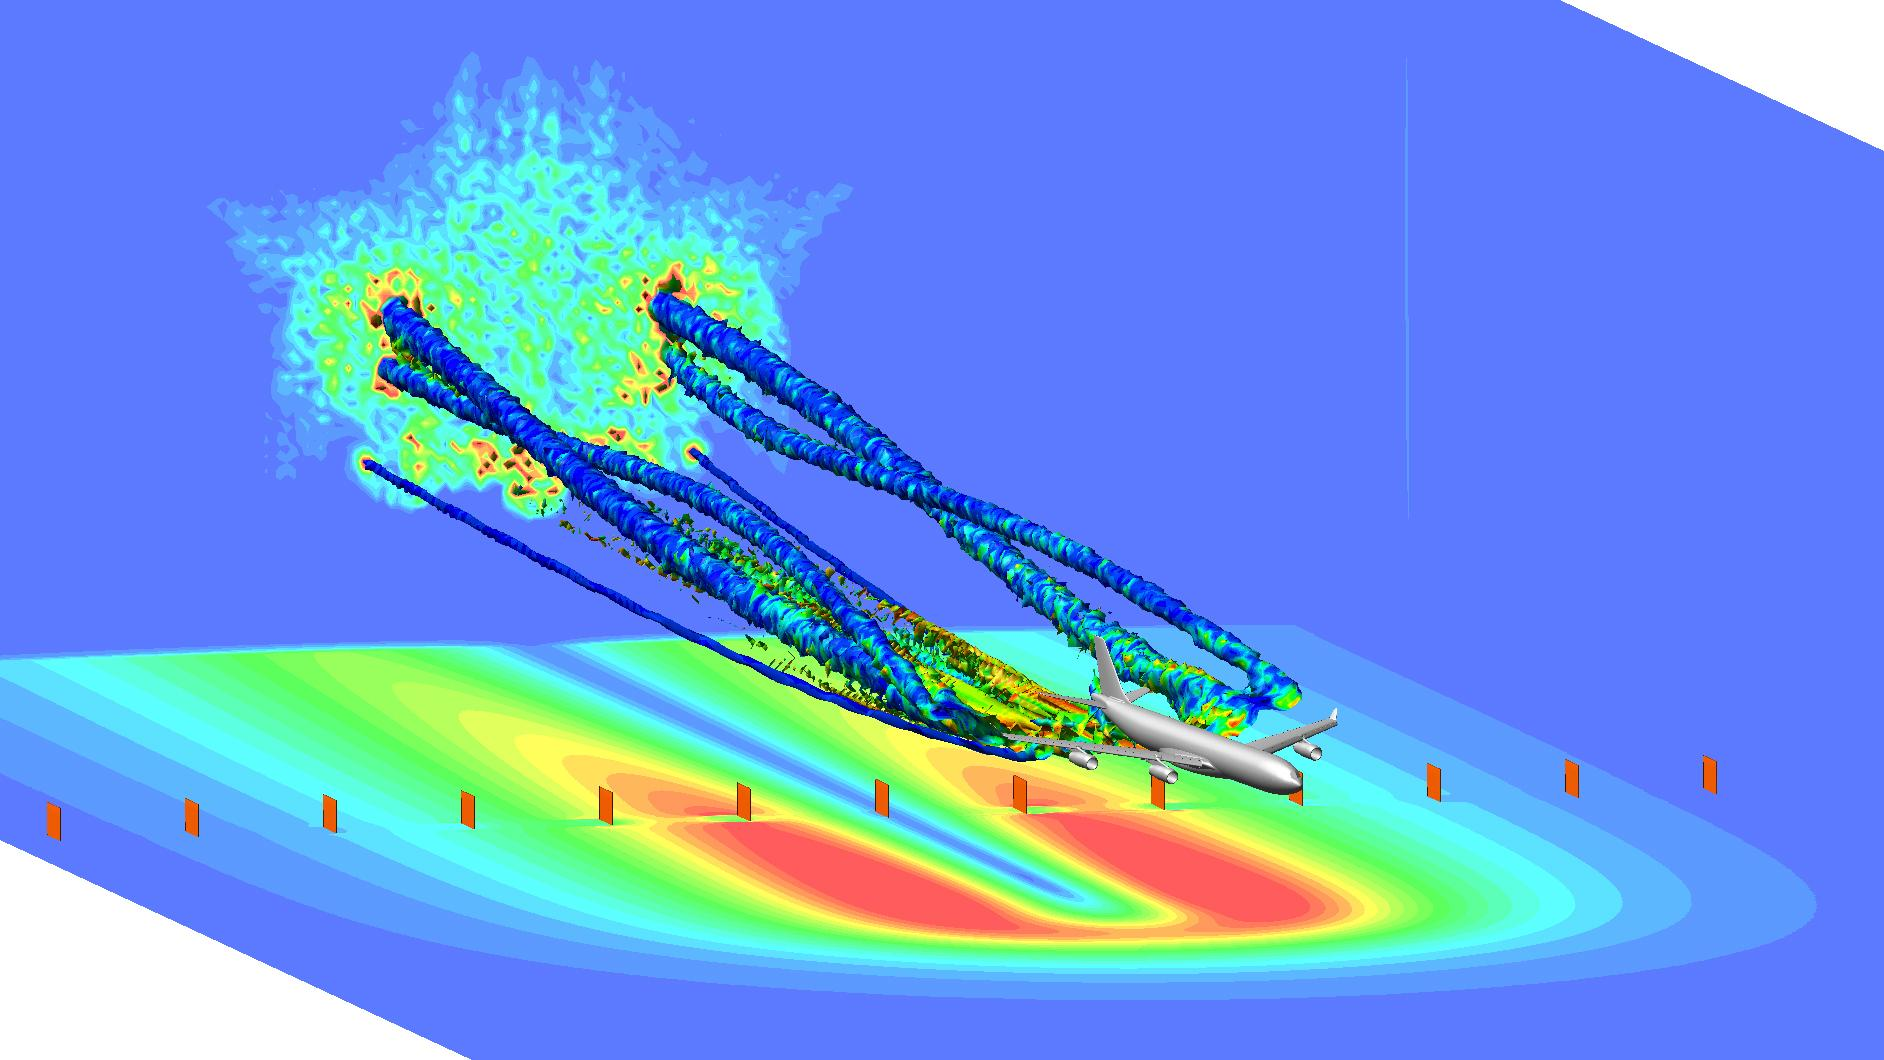
\includegraphics[width=0.8\textwidth]{papers/wirbelringe/fig/wirbelschleppen_in_der_simulation.jpg}
\caption{Simulation der Wirbelschleppenbildung eines Airbus A340 im Endanflug kurz vor der Landebahn
\cite{Wirbelringe:wirbelschleppen_in_der_simulation}. \label{Wirbelringe:fig:wirbelschleppen_in_der_simulation}}
\end{figure}

\subsection{Entstehung}
Wirbelschleppen bilden sich genau am Ende der Tragfläche aufgrund des Druckunterschieds, welcher das Flugzeug in erster Linie Fliegen lässt.
Um deren Entstehung genauer anschauen zu können gibt es nun einen kleinen Theorieausschnitt aus der Aviatik:
Setzt sich ein Flugzeug in Bewegung, so entsteht um die Flügeltragflächen ein Luftstrom.
Ein weitverbreiteter Irrglaube besagt, dass die Luft, welche über den Flügel geht, \glqq länger\grqq hat und deshalb schneller sein muss.
Dies ist jedoch nicht ganz korrekt.
Es ist vielmehr die {\em Fläche} eines einzelnen, gedachten Luftstroms, welche auf dem Flügel verkleinert wird.% TODO: Genauere Erklärung noch anfügen!
Wenn man dann mittels Kontinuitätsgleichung

\[
v_{\text{oben}}A_{\text{oben}} 
=
v_{\text{unten}}A_{\text{unten}}
\]
die Geschwindigkeiten der beiden gedachten Luftströme vergleicht, muss der Luftstrom mit Geschwindigkeit $v_{\text{oben}}$ schneller sein als $v_{\text{unten}}$.
Dies hat jetzt zur Folge, dass laut dem Satz von Bernoulli 
\begin{equation}
    p+\frac{1}{2}\rho v^2+\rho gh
    =
    const
    \label{paper:Wirbelringe:eq:Bernoulli}
\end{equation}

der Druck $p_{\text{oben}}$ kleiner sein muss als der Druck $p_{\text{unten}}$.
Nimmt man jetzt jeweils einen Punkt auf der Ober- sowie einen auf der Unterseite und setzen diese in \ref{paper:Wirbelringe:eq:Bernoulli} ein, so können sie 
\[
p_{\text{oben}}+\frac{1}{2}\rho v^2_{\text{oben}} + \rho gh_1 
=
p_{\text{unten}}+\frac{1}{2}\rho v^2_{\text{unten}}+\rho gh_2
\]
gleichgesetzt werden.
Jetzt kann angenommen werden, dass der Höhenunterschied zwischen den beiden Punkten ober und unterhalb des Flügels vernachlässigbar klein ist also \(h_1\approx h_2\).
Zudem ist die Dichte der Luft an beiden Punkten ungefähr gleich, weshalb sich der Term zu 
\[
p_{\text{oben}}+\frac{1}{2}\rho v^2_{\text{oben}} 
=
p_{\text{unten}}+\frac{1}{2}\rho v^2_{\text{unten}}
\]
vereinfacht.
Für die Druckdifferenz ergibt sich
\[
p_{\text{oben}}-p_{\text{unten}} 
=
\frac{1}{2}\rho( v^2_{\text{unten}}-v^2_{\text{oben}})
\]
und man kann erkennen, dass wenn $v_{\text{unten}} < v_{\text{oben}}$ muss $p_{\text{unten}} > p_{\text{oben}}$ sein.

Mit diesem Wissen kann auch die Entstehung der Wirbelschleppe erklärt werden. 
Es existiert also unterhalb des Flügels ein Überdruck und oberhalb ein Unterdruck.
Solange ein Flügel dazwischen ist, generiert dieser Druckunterschied einen Auftrieb, was gut und auch gewünscht ist.
Dummerweise gibt es aber eine Stelle, an der der Flügel endet und dort wirds dann auch spannend.
An der Spitze des Flügels findet nämlich ein Druckausgleich statt.
Hierbei strömt die Luft unterhalb des Flügels nach oben in das Unterdruckgebiet. 
Dabei entsteht eine Zirkulation $\Gamma$, sie zirkuliert um den ganzen Flügel.
Schlussendlich wird sie zu einer Wirbelschleppe am Flügelende.
Die entstandene Wirbelschleppe hat ein paar interessante Eigenschaften, welche in den kommenden Abschnitten behandelt werden.

\subsection{Wirbellinie}
Wie bereits im Kapitel \ref{paper:Wirbelringe:Wirbellinien} erwähnt sind Wirbellinien immer geschlossen oder enden auf Grenzflächen.
Die Wirbelschleppe jedoch hat eine ganz spezielle Wirbellinie, da diese eine Gerade von dem Flügelende bis zum Ort an dem das Flugzeug gestartet ist.
Dies klingt zunächst etwas seltsam und unglaubwürdig und natürlich ist diese Aussage auch nicht ganz korrekt.
Denn in der Realität wird sich die Wirbelschleppe natürlich irgendwann aufgrund des Luftwiderstands auflösen und somit auch die Wirbellinie verschwinden.
Also gibt es leider oder eben zum Glück keine Wirbelschleppe von Zürich nach Tokyo, wenn man mit dem Flugzeug etwaige Enkel besuchen geht.
Aber die Bedingung ist auch hier erfüllt, da die Wirbellinie am Flügelende (Grenzfläche zwischen Luft und Aluminium) startet und am Boden des Flughafens (Grenzfläche zwischen Asphalt und Luft) endet.

\begin{figure}
\centering
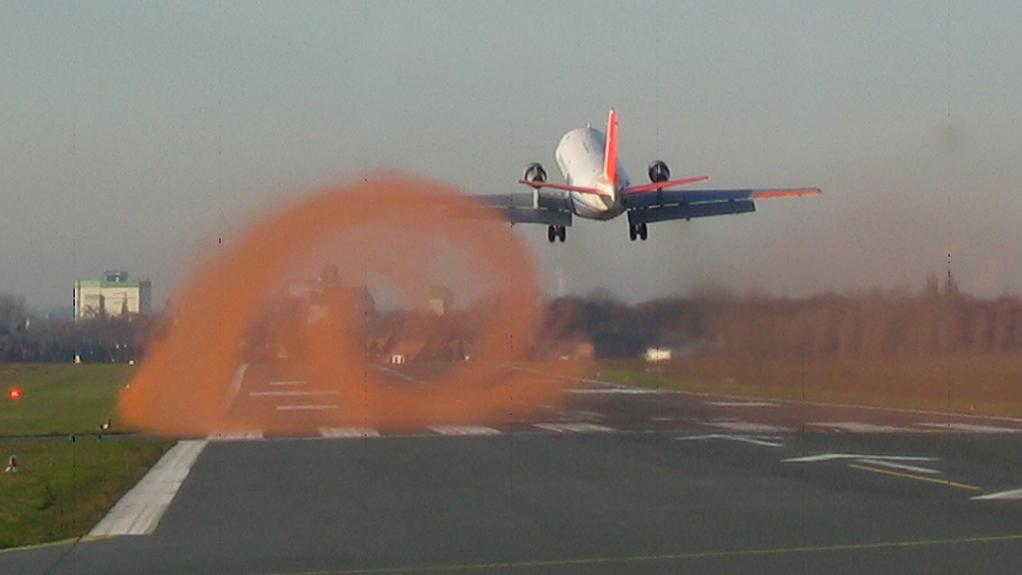
\includegraphics[width=0.8\textwidth]{papers/wirbelringe/fig/visualisierung_einer_wirbelschleppe.jpg}
\caption{Sichtbar gemachte Wirbelschleppe 
\cite{Wirbelringe:visualisierung_einer_wirbelschleppe} \label{buch:papers:Wirbelringe:fig:visualisierung_einer_wirbelschleppe}}
\end{figure}

\subsection{Problematik in der Aviatik}
Da Wirbelringe sehr stabil sind und sich nicht sofort auflösen, bleiben auch die Wirbelschleppen relativ lange bestehen.
Zudem breiten sie sich seitlich aus und sinken hinter dem Flugzeug ab.
Bei \glqq schweren\grqq Flugzeugen (ab 136 Tonnen MCTOW\footnote{maximum certified takeoff weight oder zu Deutsch: maximales Startgewicht}) \cite{Wirbelringe:WakeTurbulence} wird vorgeschrieben, dass nachfolgende Flugzeuge bis zu 3 Minuten warten müssen bevor sie starten dürfen.
Denn sollte ein Kleinflugzeug kurz nach einem solchen Flugzeug starten wird es ziemlich sicher von dessen Wirbelschleppe erfasst.
In ganz schlimmen fällen kann dies durchaus zu einem Absturz führen.
Ebenfalls muss man bedenken, dass es Energie benötigt eine solche Wirbelschleppe aufrechtzuerhalten.
Die Energie dafür wird natürlich aus den Triebwerken des Fliegers gewonnen, welcher aber eigentlich dafür gedacht war, Passagiere von A nach B zu bringen.
Deshalb finden die Airlines es grundsätzlich nicht sehr amüsant, zwei gewaltige Wirbelschleppen hinter ihren Flugzeugen herzuziehen, auch wenn es bei Schlechtwetter sehr spektakulär aussehen kann (siehe \ref{buch:papers:Wirbelringe:fig:visualisierung_einer_wirbelschleppe}). 
Findige Wissenschaftler waren deshalb auf die Idee der Winglets gestossen.
Diese sollten durch Reduktion der Zirkulation an den Flügelenden die Bildung solcher Wirbelschleppen hemmen.
Bei diesem unterfangen hatten sie auch Erfolg aber zu einem preis, welcher in der Aviatik nicht gern gesehen ist.
Durch das Anbringen solcher Winglets an den Flügelenden steigt das Leergewicht des Flugzeuges an.
Das bedeutet, dass dieses zusätzliche Gewicht wieder mehr Treibstoff verbraucht.
Wieso werden diese aber trotzdem in Kurzstreckenflugzeugen eingesetzt?
Einerseits haben Winglets zusätzlich die angenehme Eigenschaft, den Lärm eines Flugzeuges zu reduzieren.
Andererseits höhlt bekanntlich steter Tropfen den Stein.
Wenn ein Kurzstreckenflieger täglich 5-6 mal fliegt und dabei jedes Mal 1-2 \% Treibstoff spart, so summiert sich dies und wird wieder Lohnenswert für die Fluggesellschaften.
Bei Langstreckenflügen hingegen lohnen sich die Winglets noch viel mehr, da bei längerem Flug auf Reiseflughöhe (\textasciitilde10'000 m.ü.M.) auch die Wirkung der Winglets länger genutzt werden kann.
